\PassOptionsToPackage{table,usenames,dvipsnames,x11names}{xcolor}
\documentclass[english,serif,mathserif]{beamer}
\usetheme[informal]{gc3}

\usepackage[T1]{fontenc}
\usepackage[utf8]{inputenc}
\usepackage{babel}

\usepackage{gc3}

\usepackage{colortbl}
\makeatletter
\rowcolors{1}{uzh@blue!10}{white}
\makeatother

\usepackage{dcolumn}
\newcolumntype{d}[1]{D{.}{\cdot}{#1} }


\begin{document}

%% Optional Argument in [Brackets]: Short Title for Footline
\title[Databases]{A Short Introduction to Relational Databases}
\subtitle{Part 2}
\author{Riccardo Murri \texttt{<riccardo.murri@uzh.ch>}}
\date{2019-04-09}

%% Makes the title slide
\maketitle

\part{Creating tables (SQL DDL)}

\begin{frame}[fragile]
  \frametitle{Table definition (1/2)}
  Informally defined:

  \+
  \begin{quote}
    A table definition is the list of column names \\ and their associated data types.
  \end{quote}

  \+
  (For a more formal treatment, see pt.~1 of this talk.)

\end{frame}


\begin{frame}[fragile]
  \frametitle{Table definition (2/2)}

  In SQL, we write a table definition as the table name, followed by the list
  of column names (and types) within parentheses:
  \begin{sql}
    Movie(name VARCHAR(64), released DATE,
          length INTEGER,   filmType CHAR(5))
  \end{sql}
\end{frame}


\begin{frame}[fragile]
  \frametitle{Data types (1/4)}
  \smaller

  ANSI SQL includes the following string data types.

  \begin{describe}{Character strings}
    \begin{tabular}{>{\ttfamily\flushright}p{0.45\linewidth}>{\flushleft}p{0.5\linewidth}l}
      % NOTE: the extra 'l' column and associated '&' at the end of each line
      % are there to prevent an issue with LaTeX mistaking the '\\' to be part
      % of the 'p{...}' column instead of the table-row terminator...
      CHARACTER(n) \textnormal{or}~CHAR(n)
      & {fixed-width $n$-character string, padded with spaces} &
      \\
      {CHARACTER VARYING(n)} \textnormal{or}~{VARCHAR(n)}
      & {variable-width string with a maximum size of $n$ characters} &
    \end{tabular}
  \end{describe}

  \begin{describe}{Bit strings}
    \begin{tabular}{>{\ttfamily\flushright}p{0.45\linewidth}>{\flushleft}p{0.5\linewidth}l}
      % see note above re: the extra column
      BIT(n) & an array of exactly $n$ bits & \\
      BIT VARYING(n) & an array of up to $n$ bits & \\
    \end{tabular}
  \end{describe}
\end{frame}


\begin{frame}[fragile]
  \frametitle{Data types (2/4)}
  \smaller

  ANSI SQL includes the following numeric data types.

  \begin{describe}{Numbers}
    \begin{tabular}{>{\ttfamily\flushright}p{0.45\linewidth}>{\flushleft}p{0.5\linewidth}l}
      % see note above re: the extra column
      INTEGER, SMALLINT, \textnormal{and}~BIGINT & fixed-size integer numbers &\\
      FLOAT, REAL \textnormal{and} DOUBLE~PRECISION & floating-point numbers &\\
      NUMERIC(prec,scale) \textnormal{or} DECIMAL(prec,scale)
                                                 & fixed-precision numbers
                                                   % see: http://stackoverflow.com/a/759606/459543
                                                                              &\\
    \end{tabular}
  \end{describe}

  \+\smaller
  The precision is a positive integer that determines the total number of
  digits. The scale is a non-negative integer, indicating the number of digits
  after the decimal point/comma.

  \+
  For example, the number 123.45 has a precision of 5 and a scale of 2.

  % SQL provides a function to round numerics or dates, called TRUNC (in
  % Informix, DB2, PostgreSQL, Oracle and MySQL) or ROUND (in Informix, SQLite,
  % Sybase, Oracle, PostgreSQL and Microsoft SQL Server)[30]

\end{frame}


\begin{frame}[fragile]
  \frametitle{Data types (3/4)}
  \small

  ANSI SQL includes the following temporal data types.

  \begin{describe}{Time/Date}
    \begin{tabular}{>{\ttfamily\flushright}p{0.20\linewidth}>{\flushleft}p{0.75\linewidth}l}
      % see note above re: the extra column
      DATE& for date values (e.g. \texttt{DATE '2011-05-03'}) &\\
      TIME& for time values (e.g. \texttt{TIME '15:51:36'}) &\\
      TIMESTAMP& {\texttt{DATE} and \texttt{TIME} combined \\ (e.g. \texttt{TIMESTAMP '2011-05-03 15:51:36'})} &
    \end{tabular}
  \end{describe}

  \+
  The way to enter date/time \emph{constants} is by using a string prefixed with
  the word \texttt{TIME}/\texttt{DATE}/\texttt{TIMESTAMP}.

  \+ The current system date / time of the database server can be called by
  using functions \texttt{CURRENT\_DATE} / \texttt{CURRENT\_TIME} /
  \texttt{CURRENT\_TIMESTAMP}

\end{frame}


\begin{frame}[fragile]
  \frametitle{Data types (4/4)}
  \smaller

  ANSI SQL includes the following timezone-aware temporal data types.

  \begin{describe}{Time/Date}
    \begin{tabular}{>{\ttfamily\flushright}p{0.5\linewidth}>{\flushleft}p{0.45\linewidth}l}
      % see note above re: the extra column
      TIME WITH TIME ZONE \textnormal{or}~TIMETZ& same as \texttt{TIME}, but including time-zone offset &\\
      TIMESTAMP WITH TIME ZONE \textnormal{or}~TIMESTAMPTZ& same as \texttt{TIMESTAMP}, but including time-zone offset &\\
    \end{tabular}
  \end{describe}

  \+
  SQL provides ways of generating a date/time variable out of a date/time
  string, as well as for extracting the respective members (seconds, for
  instance) of such variables. See:
  \url{https://en.wikibooks.org/wiki/SQL_Dialects_Reference/Functions_and_expressions/Date_and_time_functions}
\end{frame}


\begin{frame}[fragile]
  \frametitle{CREATE TABLE}

  SQL statement \texttt{CREATE TABLE} is used to \\
  create a table in the current database:
  \begin{sql}
    CREATE TABLE Movie(name VARCHAR(64), released DATE,
                       length INTEGER,   filmType CHAR(5));
  \end{sql}

  \+
  Right after creation, the table contains no rows.
\end{frame}


\begin{frame}[fragile]
  \frametitle{CREATE TABLE (2/2)}

  {\bfseries
    There is no \emph{portable} way of reading back a table
    definition after it has been created!}

  \+
  For example, to view the schema of table {\em\ttfamily tablename} you would
  have to enter (depending on the RDBMS):

  \+
  \begin{tabular}{l>{\ttfamily}l}

    {\em RDBMS}    & {\normalfont\em command}             \\
    PostgreSQL     & {{\textbackslash}d \emph{tablename}} \\
    MySQL / MariaDB& {DESCRIBE \emph{tablename}}; \\
    SQLite         & {.schema \emph{tablename}} \\
  \end{tabular}
\end{frame}


\begin{frame}[fragile]
  \frametitle{CREATE \emph{TEMPORARY} TABLE}

  SQL statement \texttt{CREATE TEMPORARY TABLE} has exactly the same syntax as
  \texttt{CREATE TABLE}, but temporary tables are automatically deleted at the
  end of the session.

  \+
  \begin{sql}
CREATE TEMPORARY TABLE
    Movie(name VARCHAR(64), released DATE,
          length INTEGER,   filmType CHAR(5));
  \end{sql}
\end{frame}


\begin{frame}[fragile]
  \frametitle{DROP TABLE}

  To \emph{permanently} delete a table, use \texttt{DROP TABLE}:
  \begin{sql}
    DROP TABLE movie;
  \end{sql}

  \+
  An additional clause \texttt{IF EXISTS} makes the statement succeed even if
  the table had already been deleted:
  \begin{sql}
    DROP TABLE IF EXISTS movie;
  \end{sql}

\end{frame}


\part{Inserting and updating data (SQL DML)}

\begin{frame}[fragile]
  \frametitle{INSERT}

  The \texttt{INSERT} statement can be used to insert a row of values into a
  table.
  \begin{sql}
    INSERT INTO Movie(title, released, length, filmType)
    VALUES ('Star Wars', DATE '1977-05-25', 124, 'color');
  \end{sql}

  \+
  \textbf{Note:}
  \begin{itemize}
  \item
    the \texttt{INSERT} fails if the same row (or a row agreeing on
    the \emph{key} columns) is already present in the table.
  \end{itemize}

  \+
  \begin{references}
    For more details, see:
    \url{https://en.wikipedia.org/wiki/Insert_(SQL)}
  \end{references}
\end{frame}


\begin{frame}[fragile]
  \frametitle{INSERT INTO $\ldots$ SELECT}\small

  A variant of \texttt{INSERT} allows inserting into a table the results of a
  query on another table:

  \+
  \begin{sql}
    INSERT INTO lustre_u116(grp, ~size~, path)
    SELECT grp, ~size~, path FROM lustre
    WHERE usr='usr116';
  \end{sql}

  \+
  Note that:
  \begin{itemize}
  \item The schema of the table being \texttt{INSERT}'ed to must match the
    (sub)schema of columns in the \texttt{SELECT} query.
  \item There are no parentheses around the \texttt{SELECT} sub-query.
  \item No duplicate rows must be returned by the sub-query.
  \end{itemize}
\end{frame}


\begin{frame}[fragile]
  \frametitle{UPDATE}\small

  The \texttt{UPDATE} statement allows changing one or more fields in
  \emph{existing} rows.

  \begin{sql}
    -- rename user
    UPDATE lustre SET usr='rmurri' WHERE usr='usr999';

    -- alter all values in a column
    UPDATE lustre SET blksize=(4096*blksize);
  \end{sql}

  \+
  \textbf{Note:}
  \begin{itemize}
  \item The \texttt{WHERE} clause has the same syntax and semantics as its
    equivalent in the \texttt{SELECT} statement.
  \item If you omit the \texttt{WHERE} clause, \textbf{all rows will be updated!}
  \end{itemize}

  \+
  \begin{references}
    For more details, see:
    \url{https://en.wikipedia.org/wiki/Update_(SQL)}
  \end{references}
\end{frame}


\begin{frame}
  \frametitle{MERGE (1/3)}

  \begin{center} \Large
    What if you want to \\ change some fields in a row,
    \\
    \emph{or}
    \\
    add the entire row \\ if it's not already there?
  \end{center}
\end{frame}


\begin{frame}[fragile]
  \frametitle{MERGE (2/3)}\footnotesize{}

  SQL:2003 introduced the \texttt{MERGE} statement:

   \begin{sql}
MERGE INTO ~\emph{target}~ USING ~\emph{source}~ ON (~\em columns~)
  WHEN MATCHED THEN
    UPDATE SET column1 = value1 [, column2 = value2 ...]
  WHEN NOT MATCHED THEN
    INSERT (column1 [, column2 ...])
      VALUES (value1 [, value2 ...]);
 \end{sql}

 \+
 A right outer join is employed over {\ttfamily\em target} and {\ttfamily\em
   source}, then:
 \begin{itemize}
 \item
    If the \texttt{ON} field(s) in {\ttfamily\em source} matches the \texttt{ON} field(s) in {\ttfamily\em target}, then
    \texttt{UPDATE}
  \item
    If the \texttt{ON} field(s) in {\ttfamily\em source} does not match the \texttt{ON} field(s) in
    {\ttfamily\em target}, then \texttt{INSERT}
  \item
    If the \texttt{ON} field(s) does not exist in {\ttfamily\em source}
    but does exist in {\ttfamily\em target}, then no action is performed.
  \item If the \texttt{ON} field(s) does not exist in either
    {\ttfamily\em source} or {\ttfamily\em target}, then no action is performed.
  \item If multiple {\ttfamily\em source} rows match a given {\ttfamily\em target} row,
    an error is mandated by SQL:2003 standards.
 \end{itemize}
\end{frame}


\begin{frame}[fragile]
  \frametitle{MERGE (3/3)}\footnotesize

  \+ \textbf{Note:} As of today, none of the popular open-source RDBMS'es
  supports the \texttt{MERGE} statement.

  \+
  MySQL/MariaDB supports \texttt{REPLACE INTO}: first attempt an insert, and if
  that fails, delete the row (if exists) and then insert the new one.

  \+
  SQLite's \texttt{INSERT OR REPLACE INTO} works similarly.

  \+
  PostgreSQL supports merging via \texttt{INSERT INTO ... ON CONFLICT [ conflict\_target ] conflict\_action.}

  \+
  \begin{references}
    For more details, see:
    \url{https://en.wikipedia.org/wiki/Merge_(SQL)}
  \end{references}
\end{frame}


\part{Joins}
\begin{frame}
  \frametitle{Joins}

  From \href{https://en.wikipedia.org/wiki/Join_(SQL)}{Wikipedia}:

  \+
  \begin{quote}
    A SQL \texttt{JOIN} clause combines columns from one or more tables in a
    relational database {\em [$\ldots$]} by using values common to each.

    \+ ANSI-standard SQL specifies five types of JOIN: \texttt{INNER},
    \texttt{LEFT~OUTER}, \texttt{RIGHT~OUTER}, \texttt{FULL~OUTER} and
    \texttt{CROSS}.
  \end{quote}

   \+
   \begin{references}
     For more details, see:
     \url{https://en.wikipedia.org/wiki/Join_(SQL)}
   \end{references}
\end{frame}


\begin{frame}[fragile]
  \frametitle{CROSS JOIN}

  The \texttt{CROSS JOIN} operator produces the \emph{Cartesian product} of two
  relations.

  \begin{center}
    \begin{tabular}{c}
      \textbf{t1}
      \\
      \hline
      1
      \\
      2
    \end{tabular}
    {\color{gray}$\pmb\times$}
    \begin{tabular}{c}
      \textbf{t2}
      \\
      \hline
      a
      \\
      b
    \end{tabular}
    {\color{gray}$\pmb\rightarrow$}
    \begin{tabular}{cc}
      \textbf{t1} & \textbf{t2}
      \\
      \hline
      1 & a
      \\
      1 & b
      \\
      2 & a
      \\
      2 & b
    \end{tabular}

    \+
    \begin{minipage}{32ex}
    \begin{sql}
SELECT * FROM t1 CROSS JOIN t2;
    \end{sql}
  \end{minipage}
  \end{center}
\end{frame}


\begin{frame}
  \begin{center}
    \Large What if two tables have \\ the same column names?
  \end{center}
\end{frame}


\begin{frame}[fragile]
  \frametitle{INNER JOIN}

  An \texttt{INNER JOIN} returns the set of tuples from the cross product of two
  tables that satisfy a certain predicate:

  \begin{center}
    \begin{tabular}{cc}
      \rowcolor{white}\multicolumn{2}{c}{\em Table: Directors}
      \\
      \hline
      \textbf{name} & \textbf{prizeId}
      \\
      \hline
      F.~F.~Coppola & 11
      \\
      T.~Kitano & 27
    \end{tabular}
    {\color{gray}$\pmb\Join$}
    \begin{tabular}{cc}
      \multicolumn{2}{c}{\em Table: Prizes}
      \\
      \hline
      \textbf{id} & \textbf{prize}
      \\
      \hline
      27 & Leone d'Oro
      \\
      11 & Oscar
    \end{tabular}
    \\
    {\color{gray}$\pmb\downarrow$}
    \\
    \begin{tabular}{cc}
      \multicolumn{2}{c}{\em Table: Result}
      \\
      \hline
      \textbf{name} & \textbf{prize}
      \\
      \hline
      F.~F.~Coppola & Oscar
      \\
      T.~Kitano & Leone d'Oro
      \\
    \end{tabular}

    \+
    \begin{minipage}{32ex}
    \begin{sql}
SELECT name, prize
FROM directors INNER JOIN prizes
ON directors.prizeId = prizes.id ;
    \end{sql}
  \end{minipage}
  \end{center}
\end{frame}


\begin{frame}[fragile]
  \frametitle{INNER JOIN}

  An \texttt{INNER JOIN} returns the set of tuples from the cross product of two
  tables that satisfy a certain predicate.

  \+
  \begin{sql}
SELECT name, prize
FROM directors INNER JOIN prize
ON ~\HL{directors.prizeId = prizes.id}~ ;
   \end{sql}

   \+
   This is the selection predicate.

   \+
   It can contain any valid boolean expression,
   not just equality comparisons.
\end{frame}


\begin{frame}[fragile]
  \frametitle{INNER JOIN}

  An \texttt{INNER JOIN} returns the set of tuples from the cross product of two
  tables that satisfy a certain predicate:

  \+
    \begin{sql}
SELECT name, prize
FROM ~\HL{directors}~ INNER JOIN ~\HL{prizes}~
ON directors.prizeId = prizes.id ;
    \end{sql}

    \+
    The two \emph{relations} to join.

    \+
    They are referred to as \emph{left} and \emph{right} table.
    \\
    (Need not be tables: views or subqueries \\ will do as well.)
\end{frame}


\begin{frame}[fragile]
  \frametitle{INNER JOIN}

  An \texttt{INNER JOIN} returns the set of tuples from the cross product of two
  tables that satisfy a certain predicate:

  \+
    \begin{sql}
SELECT ~\HL{name, prize}~
FROM directors INNER JOIN prizes
ON directors.prizeId = prizes.id ;
    \end{sql}

    \+
    As in any \texttt{SELECT} statement, you can then project on a subset of the
    columns, in particular you can \emph{exclude} the joined columns from the
    output.
\end{frame}


\begin{frame}[fragile]
  \frametitle{Implicit INNER JOIN}

  These two \texttt{SELECT} statements are equivalent:

  \+
  \begin{sql}
-- explicit INNER JOIN
SELECT name, prize
FROM directors INNER JOIN prizes
ON directors.prizeId = prizes.id ;
    \end{sql}

  \+
  \begin{sql}
-- implicit
SELECT directors.name, prizes.prize
FROM directors, prizes
WHERE directors.prizeId = prizes.id ;
\end{sql}

  \+
  (Omitting the \texttt{WHERE} clause in the implicit syntax results in a cross join.)
\end{frame}

\begin{frame}[fragile]
  \frametitle{Self-joins}
  Self-joins are joins of a relation with (a copy of) itself.

  \+
  For example: \emph{find all pairs of film directors who have won the same prize.}

  \+
  \textbf{How would you write such a query?}
\end{frame}


\begin{frame}[fragile]
  \frametitle{Self-joins}
  Self-joins are joins of a relation with (a copy of) itself.

  \+
  For example: \emph{find all pairs of film directors who have won the same prize.}

  \+
  \alert{Use table aliases!}

  \+
\begin{sql}
SELECT ~\HL{d1.}~name, ~\HL{d2.}~name
FROM directors ~\HL{AS d1}~, directors ~\HL{AS d2}~
WHERE ~\HL{d1.}~prizeId = ~\HL{d2.}~prizeId;
  \end{sql}
\end{frame}


\begin{frame}
  \frametitle{Equi-joins and natural joins}

  A join operation is called an \emph{equi-join} if the selection predicate is a
  conjunction of equality comparisons.

  \+ The \texttt{NATURAL JOIN} is an equi-join where the \emph{implied}
  selection predicate specifies equality on all common attribute names.

  \+ (The same natural join query may return different results if table schemas
  have been altered. Avoid them: ``explicit is better than implicit''.)
\end{frame}


\begin{frame}
  \frametitle{\texttt{NULL}s, again}

  Recall that the special SQL value \texttt{NULL} makes any arithmetic or
  boolean expression undefined.

  \+
  (In particular, \texttt{NULL} does not even compare equal to itself.)

  \+ Therefore: \textbf{\texttt{INNER JOIN}s skip any row that contains a
    \texttt{NULL} value} on either side. (Unless you specifically catered for
  \texttt{NULL}s in the predicate.)
\end{frame}

\def\ojoin{\setbox0=\hbox{$\Join$}%
  \rule[0.1ex]{.27em}{.4pt}\llap{\rule[1.3ex]{.27em}{.4pt}}}
\def\leftouterjoin{\mathbin{\ojoin\mkern-5.8mu\Join}}
\def\rightouterjoin{\mathbin{\Join\mkern-5.8mu\ojoin}}
\def\fullouterjoin{\mathbin{\ojoin\mkern-5.8mu\Join\mkern-5.8mu\ojoin}}

\begin{frame}
  \frametitle{OUTER JOIN}

  In a \texttt{OUTER JOIN}, the result table retains each row, even if no other
  matching row exists.

  \+
  \begin{itemize}
  \item In a \texttt{LEFT OUTER JOIN}, every row from the \textbf{left} table is
    retained: the result is padded with \texttt{NULL} if no matching row from
    the \emph{right} table is found.
  \item A \texttt{RIGHT OUTER JOIN} does the same with \emph{left} and
    \textbf{right} reversed.
  \item In a \texttt{FULL OUTER JOIN}, rows from both sides are retained.
  \end{itemize}
\end{frame}


\begin{frame}[fragile]
  \frametitle{LEFT OUTER JOIN}

  \begin{center}
    \begin{tabular}{cc}
      \rowcolor{white}\multicolumn{2}{c}{\em Table: Directors}
      \\
      \hline
      \textbf{name} & \textbf{prizeId}
      \\
      \hline
      F.~F.~Coppola & 11
      \\
      T.~Kitano & 27
      \\
      Ed Wood & \texttt{NULL}
    \end{tabular}
    {\color{gray}$\pmb\leftouterjoin$}
    \begin{tabular}{cc}
      \multicolumn{2}{c}{\em Table: Prizes}
      \\
      \hline
      \textbf{id} & \textbf{prize}
      \\
      \hline
      27 & Leone d'Oro
      \\
      11 & Oscar
    \end{tabular}
    \\
    {\color{gray}$\pmb\downarrow$}
    \\
    \begin{tabular}{cc}
      \multicolumn{2}{c}{\em Table: Result}
      \\
      \hline
      \textbf{name} & \textbf{prize}
      \\
      \hline
      F.~F.~Coppola & Oscar
      \\
      T.~Kitano & Leone d'Oro
      \\
      Ed Wood & \texttt{NULL}
    \end{tabular}

    \+
    \begin{minipage}{32ex}
    \begin{sql}
SELECT name, prize
FROM directors LEFT JOIN prizes
ON directors.prizeId = prizes.id ;
    \end{sql}
  \end{minipage}
  \end{center}
\end{frame}


\section{Normal forms}
\begin{frame}
  \begin{center}
    {\Large\em Why are joins important?}

    \+
    {\Large Because Normal forms!}
  \end{center}
\end{frame}


\begin{frame}[fragile]
  \frametitle{Why normal forms?}
  Suppose we want to keep a database of courses being taught at the University,
  and data about their instructors (e.g., room, office hours).

  \+
  A pretty natural choice seems to have one row per course with this schema:
\begin{semiverbatim}
Courses(code, instructor, room, office_hours)
\end{semiverbatim}

  \+
  \uncover<2->{%
    But many instructors teach more than one course!  How do we solve that?
  }%

  \+
  \uncover<3->{%
    Try repeating rows: each course has a row.
  }%

  \+
  \uncover<4->{%
    \em Unfortunately, this design suffers
    from insert, update, and deletion \textbf{anomalies}.
  }%
\end{frame}


\begin{frame}
  \frametitle{Update anomalies}
  \begin{center}
    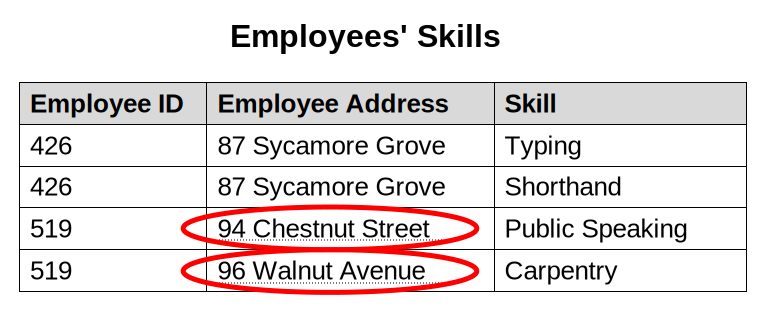
\includegraphics[width=0.8\linewidth]{update-anomaly.pdf}

    \+
    An \textbf{update anomaly}. \\
    Employee 519 is shown as \\ having different addresses on different records.

    \+
    {\tiny
      Image \& text credit: \url{https://en.wikipedia.org/wiki/Database_normalization}}
  \end{center}
\end{frame}


\begin{frame}
  \frametitle{Insertion anomalies}
  \begin{center}
    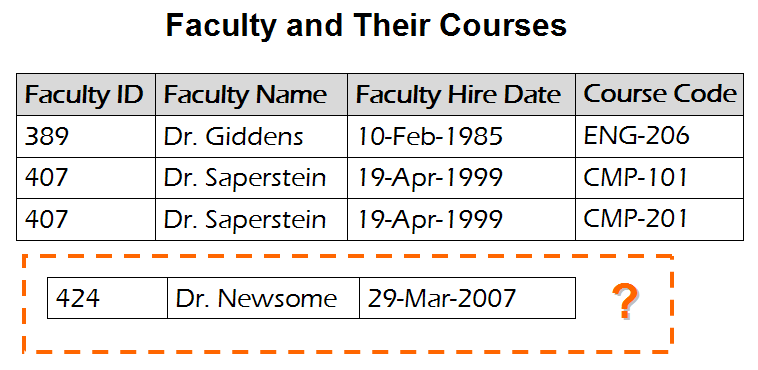
\includegraphics[width=0.8\linewidth]{insertion-anomaly.png}

    \+ An \textbf{insertion anomaly}. \\ Until the new faculty member, Dr.~Newsome, \\
    is assigned to teach at least one course, \\ his details cannot be recorded.

    \+
    {\tiny
      Image \& text credit: \url{https://en.wikipedia.org/wiki/Database_normalization}}
  \end{center}
\end{frame}


\begin{frame}
  \frametitle{Deletion anomalies}
  \begin{center}
    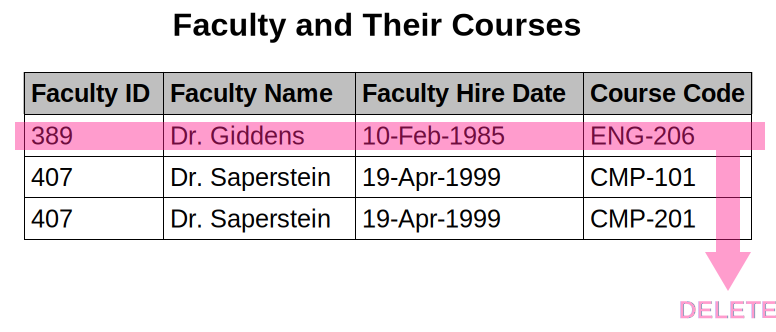
\includegraphics[width=0.8\linewidth]{deletion-anomaly.pdf}

    \+ A \textbf{deletion anomaly}. \\ All information about Dr.~Giddens is lost \\ if
    he temporarily ceases to be assigned to any courses.

    \+
    {\tiny
      Image \& text credit: \url{https://en.wikipedia.org/wiki/Database_normalization}}
  \end{center}
\end{frame}


\begin{frame}
  \frametitle{Normalization}
  Informally, problems arise when a set of data has 1-to-many or
  many-to-many interdependencies.

  \+ Normalization is a set of rules and procedures to properly design DB tables
  to minimize (or avoid) anomalies.

  \+
  Keys and functional dependencies play a fundamental role in normalization.
\end{frame}


\begin{frame}
  \frametitle{Primary Keys}

  Recall that a \emph{superkey} for a table $T$ is a set $K$ of columns such
  that no two rows of $T$ take the same values when projected over $K$.

  \+ (Equivalently: a superkey is a set of attributes within a relation whose
  values can be used to uniquely identify a tuple.)

  \+
  A \emph{candidate key} is a minimal such set.

  \+
  A \emph{primary key} is a chosen candidate key.
\end{frame}


\begin{frame}
  \frametitle{Primary Keys in SQL}

  It is possible to designate one column or a subset of columns as
  \texttt{PRIMARY KEY} in a \texttt{CREATE TABLE} statement.

  \+
  The RDBMS enforces the following constraints for a \texttt{PRIMARY KEY}:
  \begin{itemize}
  \item \texttt{UNIQUE}: projection on the set of keys cannot yield duplicate rows.
  \item \texttt{NOT NULL}: primary keys cannot take on the special value \texttt{NULL}.
  \end{itemize}

  \+ (It is however possible to designate a column as \texttt{UNIQUE} and/or
  \texttt{NOT NULL} without it being a primary key.)
\end{frame}


\begin{frame}
  \frametitle{Foreign keys}

  A \emph{foreign key} in SQL is a constraint: a column is allowed to only take
  values that are present in a specified column of another table.

  \+ A column that is referenced as a foreign key by another column must have
  been defined with a \texttt{UNIQUE} constraint (e.g., a primary key).

  \+
  It is possible to designate foreign key constraints
  in a \texttt{CREATE TABLE} statement.

  \+
  \begin{seealso}
    \url{http://www.1keydata.com/sql/sql-foreign-key.html}
  \end{seealso}
\end{frame}

% Used in the next two slides; for more details on how this is done
% with TikZ, see: http://tex.stackexchange.com/questions/9442/how-to-draw-lines-around-multiple-table-cells
%
% Introduce a new counter for counting the nodes needed for circling
\newcounter{nodecount}
% Command for making a new node and naming it according to the nodecount counter
\newcommand\tabnode[1]{\addtocounter{nodecount}{1} \tikz \node (\arabic{nodecount}) {#1};}
% Some options common to all the nodes and paths
\tikzstyle{every picture}+=[remember picture,baseline]
\tikzstyle{every node}+=[inner sep=0pt,anchor=base, minimum width=1ex,align=center,text depth=.25ex,outer sep=1.5pt]
\tikzstyle{every path}+=[thick, rounded corners]

\begin{frame}[fragile]
  \frametitle{How to represent 1-to-many relationships}

  For instance, let us consider the relation ``has directed'' between film
  directors and movies: a director typically has supervised many movies, but a
  movie only credits a single director.

  \+
  \begin{center}
    \smaller
    \begin{tabular}{lll}
      \textbf{title} & \textbf{year} & \textbf{directorId} \\
      \hline
      Star Wars    & 1977 & \tabnode{1} \\
      Pulp Fiction & 1992 & \tabnode{3} \\
      Kids return  & 1996 & \tabnode{2} \\
      Hana-Bi      & 1997 & \tabnode{2} \\
    \end{tabular}
    \hfil
    \begin{tabular}{ll}
      \textbf{id} & \textbf{name} \\
      \hline
      \tabnode{1} & G.~Lucas     \\
      \tabnode{2} & T.~Kitano    \\
      \tabnode{3} & Q.~Tarantino \\
    \end{tabular}
  \end{center}
  \begin{tikzpicture}[overlay]
    %
    \draw [orange](1.east) -- (5.west);
    \draw [yellow](2.east) -- (7.west);
    \draw [red](3.east) -- (6.west);
    \draw [red](4.east) -- (6.west);
  \end{tikzpicture}
\end{frame}


\begin{frame}[fragile]
  \frametitle{How to represent \emph{many-to-many} relationships}

  For instance, let us consider the relation ``starred in'' between actors and
  movies: actors typically star in many movies, and there is more than one actor
  starring in a given movie.

  \+
  \begin{center}
    \tiny
    \begin{tabular}{lll}
      \textbf{title} & \textbf{year} & \textbf{id} \\
      \hline
      Lawrence of Arabia & 1962 & \tikz \node (m4l) {4}; \\
      Star Wars          & 1977 & \tikz \node (m1l) {1}; \\
      The Blues Brothers & 1980 & \tikz \node (m3l) {3}; \\
      Hana-Bi            & 1997 & \tikz \node (m2l) {2}; \\
    \end{tabular}
    \hfil
    \begin{tabular}{ll}
      \textbf{mId} & \textbf{aId} \\
      \hline
      \tikz \node (m1r1) {1}; & \tikz \node (a1l1) {1}; \\
      \tikz \node (m1r2) {1}; & \tikz \node (a3l1) {3}; \\
      \tikz \node (m2r1) {2}; & \tikz \node (a2l1) {2}; \\
      \tikz \node (m3r1) {3}; & \tikz \node (a3l2) {3}; \\
      \tikz \node (m3r2) {3}; & \tikz \node (a4l1) {4}; \\
      \tikz \node (m4r1) {4}; & \tikz \node (a1l2) {1}; \\
    \end{tabular}
    \hfil
    \begin{tabular}{ll}
      \textbf{id} & \textbf{name} \\
      \hline
      \tikz \node (a1r) {1}; & A.~Guinnes   \\
      \tikz \node (a2r) {2}; & T.~Kitano    \\
      \tikz \node (a3r) {3}; & C.~Fisher    \\
      \tikz \node (a4r) {4}; & J.~Belushi   \\
    \end{tabular}
  \end{center}
  \begin{tikzpicture}[overlay]
    % connections between left and center table
    \draw [orange](m4l.east) -- (m4r1.west);
    \draw [yellow](m3l.east) -- (m3r1.west);
    \draw [yellow](m3l.east) -- (m3r2.west);
    \draw [red](m2l.east) -- (m2r1.west);
    \draw [pink](m1l.east) -- (m1r1.west);
    \draw [pink](m1l.east) -- (m1r2.west);
    % connections between center and right table
    \draw [pink](a1l1.east) -- (a1r.west);
    \draw [pink](a1l2.east) -- (a1r.west);
    \draw [red](a2l1.east) -- (a2r.west);
    \draw [orange](a3l1.east) -- (a3r.west);
    \draw [orange](a3l2.east) -- (a3r.west);
    \draw [yellow](a4l1.east) -- (a4r.west);
\end{tikzpicture}
\end{frame}


\begin{frame}
  \frametitle{Normal forms}\small

  These ways of representing $1 \to N$ and $N \to M$ relationships generally
  produce relations in \emph{third normal form} (3NF).

  \begin{describe}{1NF}
    \begin{itemize}
    \item Column values are \emph{atomic}
    \item No repeated columns (or groups thereof)
    \item Each table has a primary key
    \end{itemize}
  \end{describe}

  \begin{describe}{2NF}
    Each column must depend on the \emph{entire} primary key
  \end{describe}

  \begin{describe}{3NF}
    Each column must depend \emph{directly} on the primary key.
  \end{describe}

  \begin{seealso}
    \url{http://www.troubleshooters.com/littstip/ltnorm.html}
  \end{seealso}
\end{frame}


\part{Appendix}
\begin{frame}
  \frametitle{References}

  Pagh, R.: ``Introduction to Database Systems'',
  \url{http://www.itu.dk/people/pagh/IDB05/}

  \+
  Codd, E.~F.: ``A relational model for large shared data banks'', \emph{Comm.
  ACM} 13:6, pp.~377--387, 1970
\end{frame}


\end{document}


%%% Local Variables:
%%% mode: latex
%%% TeX-master: t
%%% End:
